% deck.tex - 决赛进展汇报 (31 pages), mirrors report/sections/*.tex, shorter.
% Build: cd .. && make slides   (tectonic, engine=xetex via ctexbeamer)
\documentclass[aspectratio=169,11pt]{ctexbeamer}

\makeatletter
\def\input@path{{./theme/}{./}}
\makeatother

\usepackage{graphicx}
\usepackage{booktabs}
\usepackage{array}

\usetheme{posad}
% CANONICAL NUMBER SET. Direction = Starry/Linux (higher=better unless a time). \abl{}=pending ablation run.
% Board-measured, 3-rep medians from the 2026-08-12 ablation; frozen Linux 6.1.43-rockchip baseline.
\newcommand{\nCpuTEight}{4987}          \newcommand{\nCpuTEightLin}{5222}   \newcommand{\nCpuTEightRatio}{0.96}
\newcommand{\nLadderBase}{160}      \newcommand{\nLadderA}{3668} \newcommand{\nLadderB}{3991}
\newcommand{\nLadderFloor}{361} \newcommand{\nLadderPlace}{4987} \newcommand{\nLadderOcc}{4995} \newcommand{\nLadderCoalesce}{3523}
\newcommand{\nAfive}{359}  \newcommand{\nAfiveLin}{349}  \newcommand{\nAfiveRatio}{1.03}
\newcommand{\nAseven}{896} \newcommand{\nAsevenLin}{962} \newcommand{\nAsevenRatio}{0.93}
\newcommand{\nThpFT}{0.030} \newcommand{\nThpFTLin}{0.086} \newcommand{\nThpRatio}{2.87}
\newcommand{\nGetpid}{431} \newcommand{\nGetpidLin}{167} \newcommand{\nGetpidRatio}{2.6}
\newcommand{\nWake}{8} \newcommand{\nWakeLin}{6}
\newcommand{\nTtfi}{9.83} \newcommand{\nTtfiLin}{11.28}
\newcommand{\nMemBWWrite}{34330} \newcommand{\nMemBWWriteLin}{56046} \newcommand{\nMemBWWriteRatio}{0.61}
\newcommand{\nMemBWMemcpyRatio}{0.36} \newcommand{\nMemBWAggRatio}{0.24}
\newcommand{\nSchRps}{339} \newcommand{\nSchRpsLin}{199} \newcommand{\nSchRpsRatio}{1.71}
\newcommand{\nMemBwTwo}{0.78}
\newcommand{\nHackT}{10.2} \newcommand{\nDvfsAseven}{2126} \newcommand{\nDvfsAsevenTop}{2256} \newcommand{\nDvfsAfive}{1881}
\newcommand{\nPerCoreRatio}{0.98}
% 推理链路（初赛，已在板上验证）
\newcommand{\nEteDefault}{162.7} \newcommand{\nEteBig}{55.2} \newcommand{\nEteBigLin}{25.8}
\newcommand{\nInferTennis}{11.75} \newcommand{\nInferTennisLin}{11.4}
\newcommand{\nRgaSpeedup}{7.4} \newcommand{\nAffinitySpeedup}{3}
\newcommand{\nMutexRatio}{1.76}
% 上游贡献足迹：自初赛至今，本队三名成员向 rcore-os/tgoskits 提交的 PR（gh 实测 2026-08-13）。
% 90 merged = 47 (队长) + 18 + 25；122 opened = 90 merged + 19 open + 13 closed；决赛期(07-01+) 新增 24 merged + 19 open。
\newcommand{\nPRMerged}{90} \newcommand{\nPROpened}{122} \newcommand{\nPRInflight}{19} \newcommand{\nPRFinalsMerged}{24}
% StarryOS 优化前基线（before），for 前 -> 后 -> Linux 三段对照 (from report ladders/baselines).
\newcommand{\nCpuTEightBefore}{160}   % boot-freq, placement off (= \nLadderBase)
\newcommand{\nGetpidBefore}{1200}
\newcommand{\nWakeBefore}{1042}
\newcommand{\nSchRpsBefore}{231}
\newcommand{\nMemBWWriteBefore}{15040}   % pre wake-spread (0.27x Linux)
\newcommand{\nTtfiBefore}{19.22}
\newcommand{\nMutexBefore}{1.69} \newcommand{\nMutexAfter}{0.85} \newcommand{\nMutexLin}{0.481}
\newcommand{\nAfiveBefore}{251} \newcommand{\nAsevenBefore}{693}   % freq-limited pre-align (~0.72x Linux)
\newcommand{\nThpFTBefore}{0.8 到 1.3}
% Removed dead placeholders \nCpuTfour (sysbench cpu 4-thread never run — harness does only 1T/8T)
% and \nThreadsTEight (sysbench threads --threads=8 hard-hangs StarryOS, #59 wake-storm); neither was
% ever referenced in prose, so both were non-rendering. See sysbench-board ABLATION.md / CAMPAIGN_LOG.md.

\graphicspath{{../figures/out/}}

% Some WIP figures (F03/F09/F14/F16/F20/F21) carry a ~25px white border; trim it
% so they sit natively on the dark canvas (25bp = 25px at graphicx's 72dpi default).
\newcommand{\gfxt}[2][\linewidth]{\includegraphics[width=#1,trim=25 25 25 25,clip]{#2}}

% verdict coloring helpers
\newcommand{\vgood}[1]{{\color{teal}#1}}      % 领先
\newcommand{\vwarn}[1]{{\color{amber}#1}}      % 外因 / 进行中 / 仍有差距
\newcommand{\vmut}[1]{{\color{muted}#1}}       % 弱化
\newcommand{\headline}[1]{{\sffamily\bfseries\color{teal}#1}}
\newcommand{\ours}[1]{\textbf{#1}}
\definecolor{skyblue}{HTML}{5B9BFF}
\newcommand{\vport}[1]{{\color{skyblue}#1}}   % 移植·使能上游

\begin{document}
% ============================== 1 封面 ==============================
\begin{frame}[plain]
  \vfill\centering
  {\sffamily\bfseries\color{ink}\LARGE 面向边缘智能的 AIOS 设计与优化}\\[6pt]
  {\color{teal}\rule{0.46\paperwidth}{1pt}}\\[10pt]
  {\sffamily\color{teal}\large 决赛进展汇报}\\[14pt]
  {\color{ink}\footnotesize 以一个真实的边缘 AI 机器人为牵引，将 StarryOS 在 RK3588 上做到对 Linux 逐轴对等乃至反超，}\\[2pt]
  {\color{ink}\footnotesize 成果全部回馈上游 \texttt{rcore-os/tgoskits}（累计 \nPRMerged{} 个 PR 已合并）。}\\[16pt]
  {\sffamily\color{muted}\large Team Posad\quad·\quad 清华大学}\\[8pt]
  {\color{muted}\footnotesize RK3588 / OrangePi-5-Plus\quad·\quad 基线 \texttt{rcore-os/tgoskits} dev @73409e079\quad·\quad 2026-08}
  \vfill
\end{frame}

% ============================== 7 网球机器人与拾球回路 ==============================
\begin{frame}
  \navsegment{1}
  \frametitle{网球机器人与拾球回路}
  \begin{columns}[T]
    \begin{column}{0.54\textwidth}
      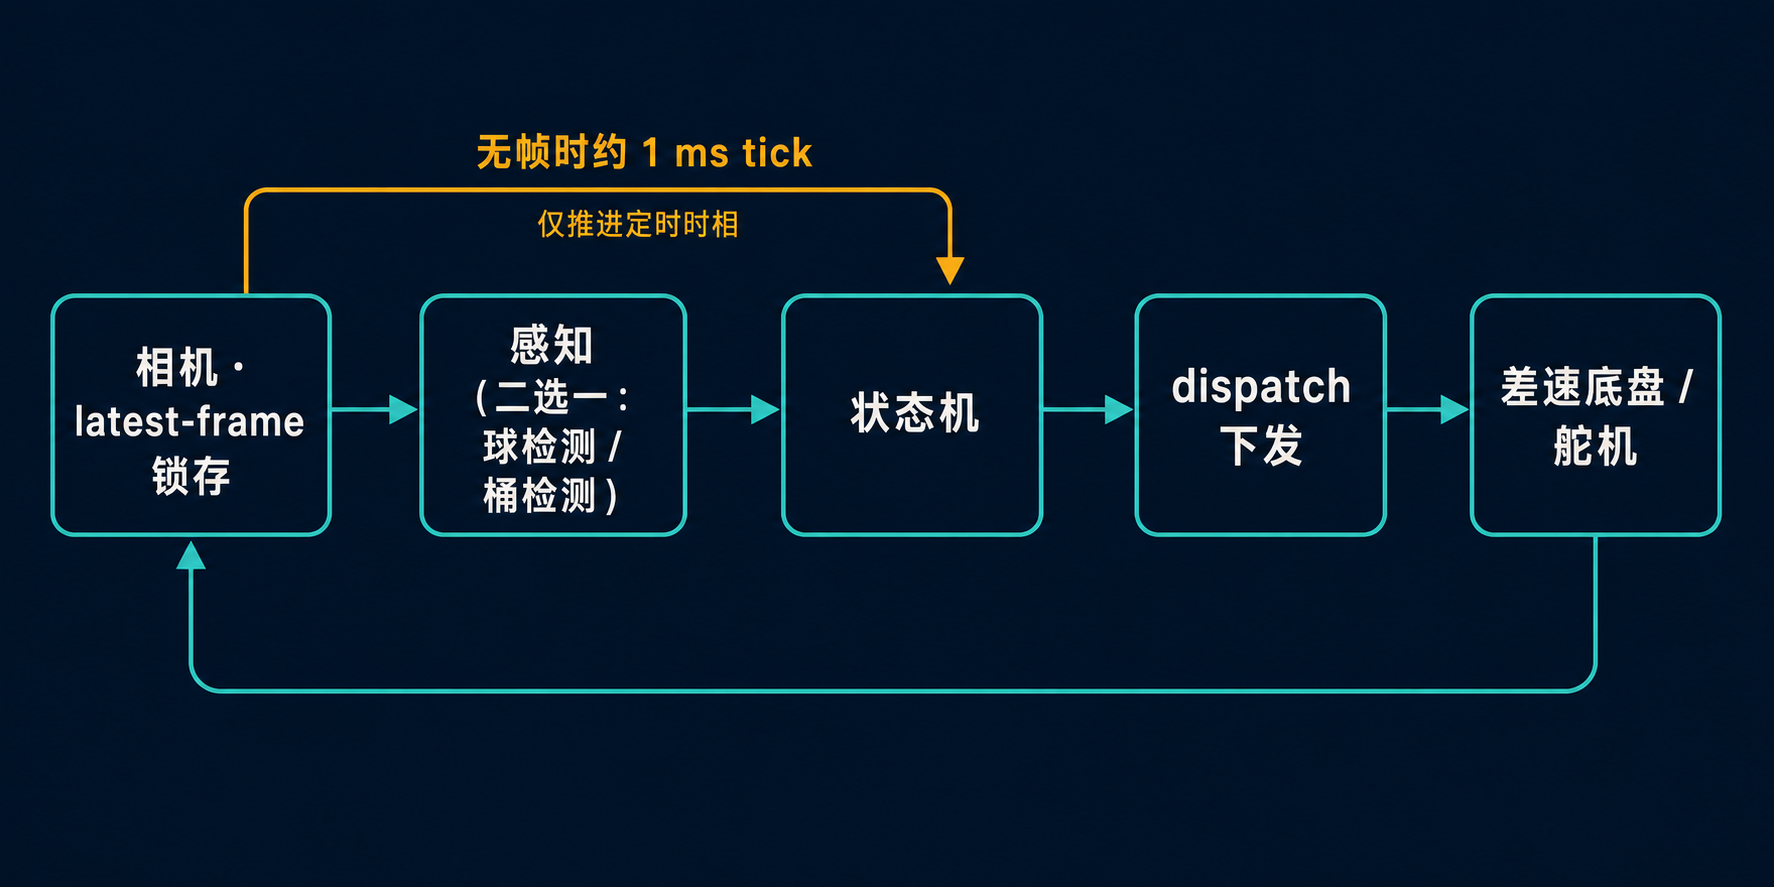
\includegraphics[width=\linewidth]{F19.png}
    \end{column}
    \begin{column}{0.43\textwidth}
      \begin{itemize}
        \item 闭环起于相机成帧，依次经 JPU 解码、RGA 预处理、NPU 推理，直至定位与运动控制，再返回相机
        \item 帧到指令延迟即闭环运行一周的端到端时间
        \item 追球交由 NPU 上的单类 YOLOv8，寻桶采用整型 HSV 红色掩膜
        \item 感知结果送入纯逻辑状态机，生成底盘与舵机指令
      \end{itemize}
    \end{column}
  \end{columns}
  \advance{机器人是内核侧工作的应用载体}{感知到控制闭环：相机 → JPU → RGA → NPU → 定位 → 运动}
\end{frame}

% ============================== H 从初赛到决赛 ==============================
\begin{frame}
  \navsegment{1}
  \frametitle{从初赛到决赛：从机器人推理到整个操作系统}
  \begin{columns}[T]
    \begin{column}{0.48\textwidth}
      {\headline{初赛}}\smallskip
      \begin{itemize}
        \item 把网球拾取机器人的操作系统由 C 语言的 Linux 迁移到 Rust 实现的 StarryOS
        \item 优化机器人的视觉推理链路，使端到端推理在真机上追平 Linux（下页详述）
      \end{itemize}
    \end{column}
    \begin{column}{0.48\textwidth}
      {\headline{决赛}}\smallskip
      \begin{itemize}
        \item 命题扩展为整机对等：让整个 StarryOS 作为通用 OS，在调度、内存、频率、启动等子系统上也对 Linux 逐轴对齐
        \item 机器人成为众多负载之一，考核操作系统的通用能力
      \end{itemize}
    \end{column}
  \end{columns}
  \vspace{1.5mm}
  {\color{muted}\footnotesize 工作量以回馈上游 \texttt{rcore-os/tgoskits} 计量（自初赛至今累计；决赛期新增 \nPRFinalsMerged{} 已合并 + \nPRInflight{} 在审）：}
  \begin{center}\setlength{\tabcolsep}{22pt}
  \begin{tabular}{ccc}
    {\Large\color{teal}\bfseries \nPRMerged} & {\Large\color{teal}\bfseries \nPROpened} & {\Large\color{teal}\bfseries \nPRInflight}\\[2pt]
    {\footnotesize\color{muted}PR 已合并} & {\footnotesize\color{muted}PR 累计提交} & {\footnotesize\color{muted}PR 评审中}\\
  \end{tabular}
  \end{center}
  \vspace{-0.5mm}
  {\color{muted}\footnotesize 覆盖系统调用/进程/信号、调度/大小核、内存/分页、观测 perf、RGA/JPU/NPU 与显示驱动、网络、虚拟化、板级；另自建 QEMU RKNPU 功能级模型，全部经 RK3588 真机验证。}
  \advance{初赛：机器人推理追平 Linux}{决赛：整个 OS 对 Linux 逐轴对等，全部成果回馈上游（累计 \nPRMerged{} 个 PR 已合并）}
\end{frame}

% ============================== KMAP 内核贡献全景 ==============================
\begin{frame}
  \navsegment{1}
  \frametitle{自底向上：本队贡献贯穿整个软件栈}
  \centering
  \includegraphics[width=\linewidth,height=0.80\textheight,keepaspectratio]{Fkmap.png}
\end{frame}

% ============================== 19b 视觉推理链路优化 ==============================
\begin{frame}
  \navsegment{1}
  \frametitle{视觉推理链路：重型模型 6.3\texttimes\ 收窄至 2.1\texttimes，小模型追平 Linux}
  \begin{columns}[T]
    \begin{column}{0.52\textwidth}
      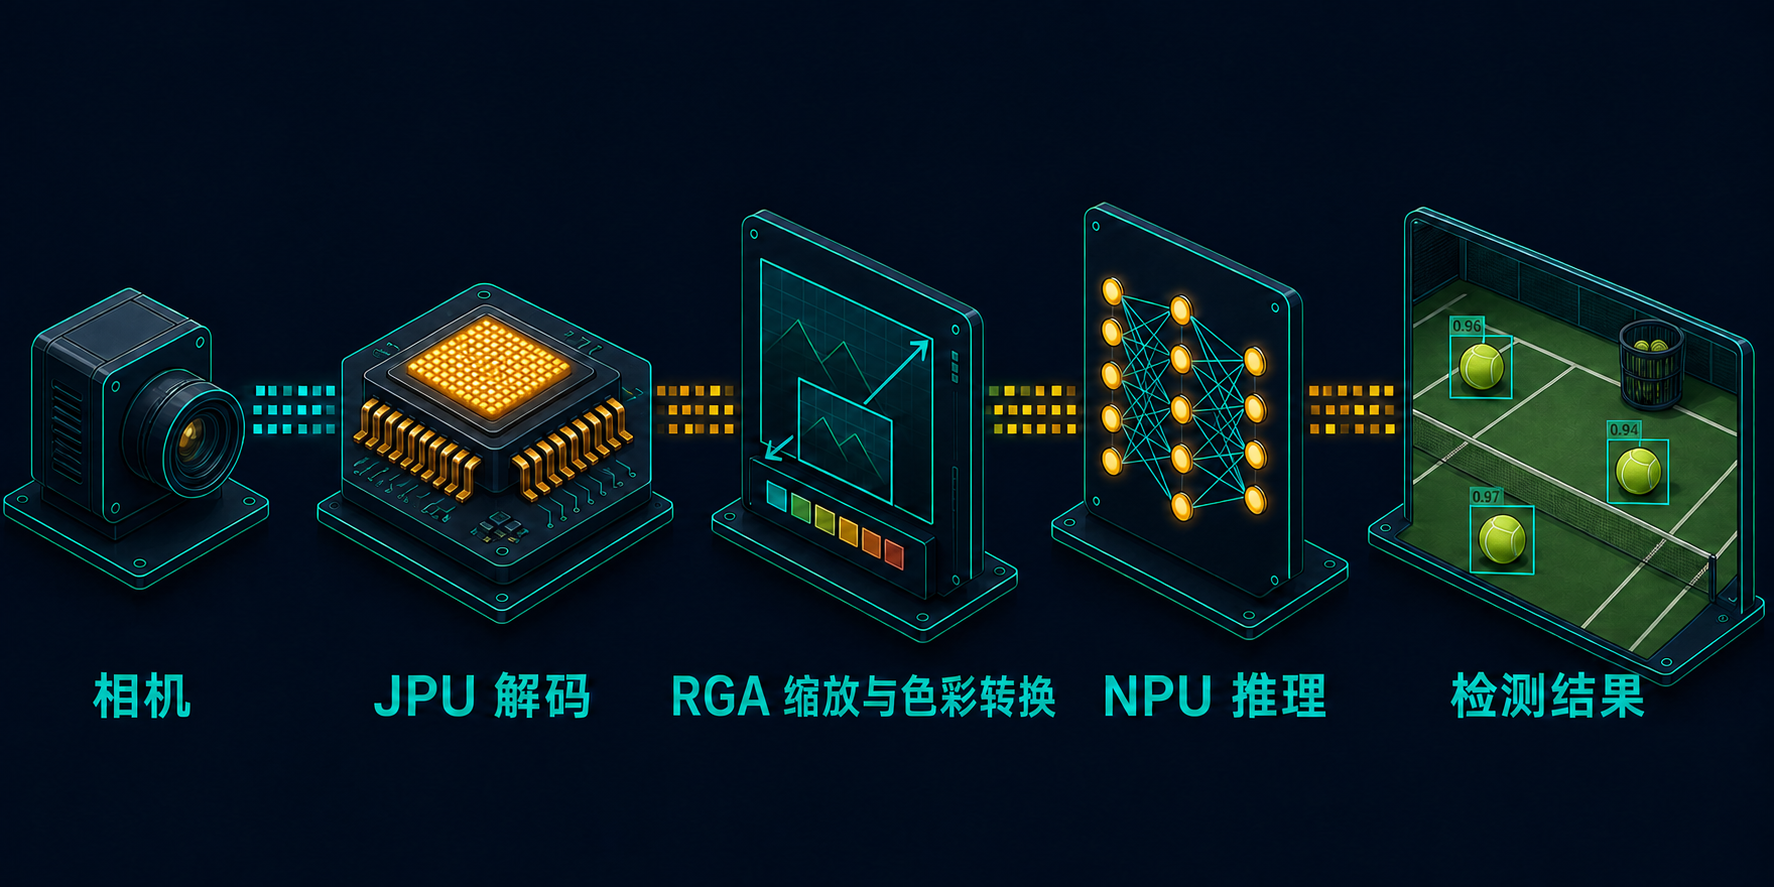
\includegraphics[width=\linewidth]{Fvision.png}
    \end{column}
    \begin{column}{0.45\textwidth}
      \begin{itemize}
        \item 同一份 ELF 两侧对测，StarryOS 起点端到端落后 Linux 约 6.3 倍，热点散在链路各阶段
        \item 绑定 A76 大核：640×640 端到端 \nEteDefault$\to$\nEteBig\,ms，三大 CPU 阶段各降约 3 到 5 倍
        \item 整数取回路径（\texttt{want\_float=0}）使 \texttt{outputs\_get} 约 12$\to$1\,ms，285 张测图逐张一致
        \item 原生 ReLU 模型将 480×640 p50 30.6$\to$\nInferTennis\,ms 追平 Linux，再加 RGA 零拷贝逐帧命令降到约 9.65\,ms
      \end{itemize}
    \end{column}
  \end{columns}
  \advance{小模型上曾落后 Linux 约 2.68 倍}{绑核 + 整数取回 + 原生 ReLU 模型 $\to$ \nInferTennis\,ms 与 Linux 持平}
\end{frame}

% ============================== 21b F01 对等仪表盘（前 -> 后 -> Linux） ==============================
\begin{frame}
  \navsegment{1}
  \frametitle{跨子系统对 Linux 的性能追平：优化前 $\to$ 优化后}
  \centering
  \includegraphics[width=\linewidth,height=0.80\textheight,keepaspectratio]{F01_deck.png}
  \advance{每项从优化前到优化后向 Linux 基线追平}{青色达到或超过 Linux，橙色分持平与仍有差距两档}
\end{frame}

% ============================== 22 按轴诚实图例 ==============================
\begin{frame}
  \navsegment{1}
  \frametitle{对 Linux 的完整基准结果（StarryOS 优化前 $\to$ 后）}
  \scriptsize
  \begin{tabular}{@{}l r r r l@{}}
    \toprule
    轴（单位） & 优化前 & 优化后 & Linux & 判定 \\
    \midrule
    THP first-touch (s) & \nThpFTBefore & \nThpFT & \nThpFTLin & \vgood{领先 \nThpRatio×} \\
    启动 TTFI (s) & \nTtfiBefore & \nTtfi & \nTtfiLin & \vgood{领先} \\
    A55 单核 (ev/s) & 约 \nAfiveBefore & \nAfive & \nAfiveLin & \vgood{领先 \nAfiveRatio×} \\
    schbench RPS & \nSchRpsBefore & \nSchRps & \nSchRpsLin & \vgood{反超 \nSchRpsRatio×} \\
    A76 单核 (ev/s) & 约 \nAsevenBefore & \nAseven & \nAsevenLin & 持平 \nAsevenRatio× \\
    cpu 八线程 (ev/s) & \nCpuTEightBefore & \nCpuTEight & \nCpuTEightLin & 持平 \nCpuTEightRatio× \\
    唤醒 p50 (µs) & \nWakeBefore & \nWake & \nWakeLin & 持平 \\
    getpid (ns) & \nGetpidBefore & \nGetpid & \nGetpidLin & 收窄 \nGetpidRatio× \\
    mutex 8T (s) & \nMutexBefore & \nMutexAfter & \nMutexLin & 收窄 \nMutexRatio× \\
    内存写 (MiB/s) & \nMemBWWriteBefore & \nMemBWWrite & \nMemBWWriteLin & 收窄 \nMemBWWriteRatio× \\
    \bottomrule
  \end{tabular}
  \par\smallskip
  {\color{muted}\scriptsize “收窄”指相对 Linux 的差距已大幅缩小（getpid 由 7$\times$ 收至 \nGetpidRatio$\times$，mutex 由 3.5$\times$ 收至 \nMutexRatio$\times$）；内存写受 DDR 变频固件限制。hackbench 的 \texttt{-T}／\texttt{-P} 比值经无锁用户拷贝快路径恢复到约 1（回到 Linux 形态）。}
  \advance{一图看清对 Linux 的位置}{十个轴：领先 THP/TTFI/A55/schbench，其余持平或收窄}
\end{frame}

% ============================== 9 观测 perf + ftrace ==============================
\begin{frame}
  \navsegment{2}
  \frametitle{观测能力：硬件 PMU perf 与 ftrace}
  \begin{itemize}
    \item 前页的对等结论均建立在测量之上，而测量依赖工具；决赛前 StarryOS 尚无基于硬件 PMU 的 perf，热点难以定位到层
    \item 构建一整套硬件 PMU perf：单核 PMUv3、big.LITTLE 分簇、软件与 cache 事件、事件组、调用栈、kprobe/tracepoint、ftrace
    \item 未经修改的上游 perf 6.1.0 二进制直接产出 \texttt{perf.data}、\texttt{report} 与 \texttt{top}；板级 big.LITTLE 矩阵 39/0、特性矩阵 56/0
    \item 受硬件限制的 PEBS 与 BRBE 类特性，按 Linux 在同一 SoC 上的行为如实拒绝，未伪造读数
  \end{itemize}
  \smallskip
  {\color{muted}\footnotesize ftrace 全量函数跟踪在真实 8 核开发板活锁（QEMU 因 smp1 未暴露），过滤式函数跟踪为板上与 QEMU 均实用的模式。}
  \advance{测量需要工具}{硬件 PMU perf + ftrace 上板，56/0，直接运行上游 perf 二进制}
\end{frame}

% ============================== 10 调度 cpu 对等阶梯（招牌） ==============================
\begin{frame}
  \navsegment{2}
  \frametitle{调度：sysbench cpu 对等阶梯}
  \begin{columns}[T]
    \begin{column}{0.56\textwidth}
      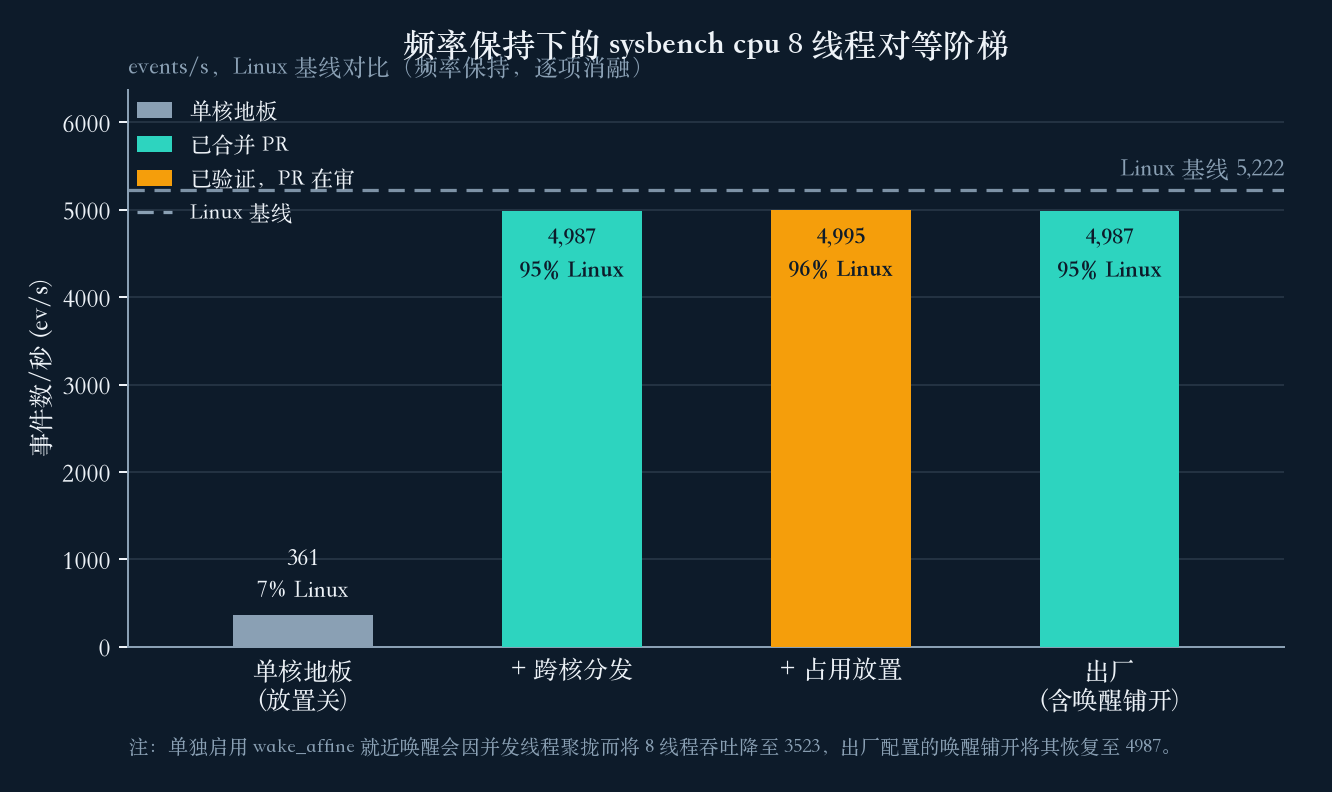
\includegraphics[width=\linewidth]{F04.png}
    \end{column}
    \begin{column}{0.41\textwidth}
      \begin{itemize}
        \item 决赛初整机压在单个 A55，八线程仅 \nCpuTEightBefore\,ev/s，落后 Linux 约三十倍（下图为频率固定下的隔离阶梯，地板 \nLadderFloor）
        \item 固定顶频以隔离放置层：跨核分发（\#1656）把八线程由单核地板 \nLadderFloor 抬到 \nLadderPlace\,ev/s，为最关键一层
        \item 叠加占用感知放置续进至 \nLadderOcc\,ev/s，增益已属小幅；出厂配置八线程 \nCpuTEight\,ev/s，为 Linux \nCpuTEightLin 的 \nCpuTEightRatio 倍，判定持平
      \end{itemize}
    \end{column}
  \end{columns}
  \advance{整机压在单个小核、落后约三十倍}{跨核分发 + 占用放置 + 顶频 $\to$ \nCpuTEightRatio× Linux（持平）}
\end{frame}

% ============================== 13 内存 THP first-touch 领先 ==============================
\begin{frame}
  \navsegment{2}
  \frametitle{内存：THP first-touch（领先）}
  \begin{columns}[T]
    \begin{column}{0.54\textwidth}
      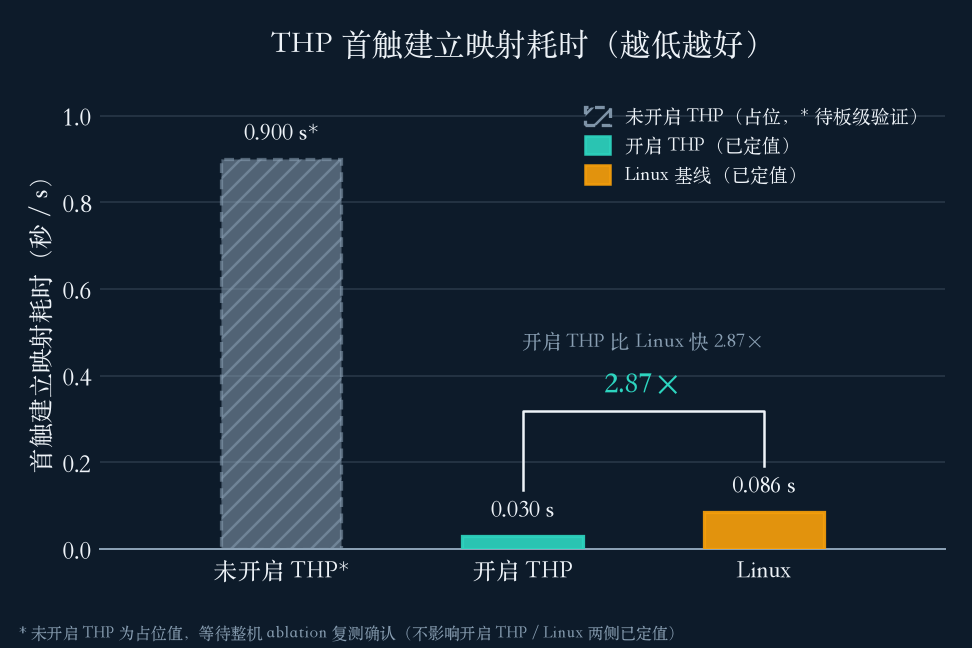
\includegraphics[width=\linewidth]{F08.png}
    \end{column}
    \begin{column}{0.43\textwidth}
      \begin{itemize}
        \item 首触路径慢：128\,MB fault-in 需 0.8 到 1.3\,s，Linux \nThpFTLin\,s，逐页约 9 到 15 倍
        \item 三级压缩：新建映射跳过广播 TLB flush、aarch64 \texttt{dc zva} 块清零、THP-lite 2\,MB 私有匿名提升
        \item 128\,MB 私有匿名首触（2\,MB THP-lite 提升）降至 \nThpFT\,s，Linux \nThpFTLin\,s，快 \nThpRatio 倍（领先）
        \item 收益来自硬件层面（更少 TLB 广播、块清零、每 2\,MB 少 512 次缺页），Linux 侧缺乏等价用户态手段
      \end{itemize}
    \end{column}
  \end{columns}
  \advance{首触逐页慢 Linux 约十倍}{三级压缩 $\to$ THP 首触 \nThpFT\,s，快 Linux \nThpRatio×（领先）}
\end{frame}

% ============================== 16 启动 TTFI 领先 ==============================
\begin{frame}
  \navsegment{2}
  \frametitle{启动：首帧推理 TTFI（领先）}
  \begin{columns}[T]
    \begin{column}{0.52\textwidth}
      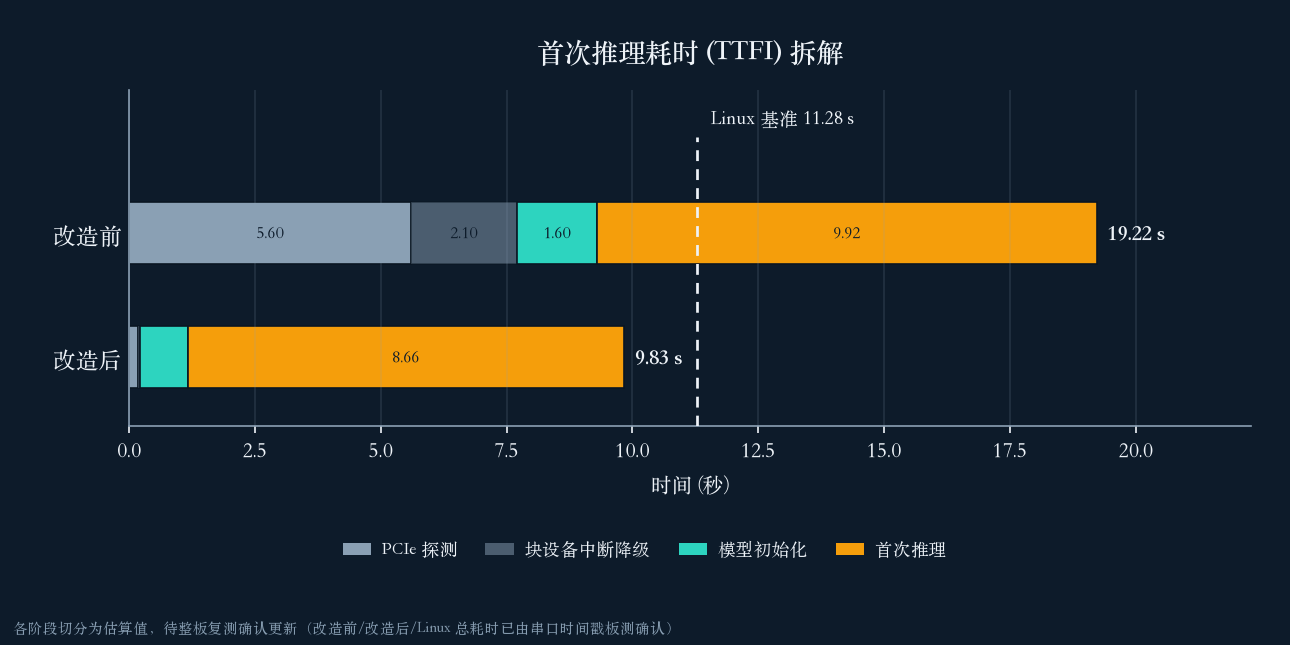
\includegraphics[width=\linewidth]{F11.png}
    \end{column}
    \begin{column}{0.45\textwidth}
      \begin{itemize}
        \item 口径：内核自 U-Boot 接管起至 live 首帧 RKNN 推理完成
        \item 提交版本 19.22\,s 慢 Linux 约 1.7 倍；经根因定位与约十一处公平改动降至 \nTtfi\,s，优于 Linux \nTtfiLin\,s（领先）
        \item 内核侧两段：PCIe 空槽串行探测约 5.6\,s（次核前置 + FDT 借用 + 空槽快返），块 IO 完成中断回退约 2.1\,s
        \item 应用侧最大一段：相机边流边初始化使 rknn\_init 饥饿，先加载模型再启相机将 model\_init 由 16870 降至 140\,ms
      \end{itemize}
    \end{column}
  \end{columns}
  \advance{提交版 TTFI 慢 Linux 约 1.7 倍}{根因定位降至 \nTtfi\,s 领先，机制为精简 init 相对 systemd bringup 的优势}
\end{frame}

% ============================== 18 QEMU NPU 模型 + 模型协同 ==============================
\begin{frame}
  \navsegment{2}
  \frametitle{QEMU RKNPU 设备模型与机器人检测模型的协同优化}
  \begin{columns}[T]
    \begin{column}{0.54\textwidth}
      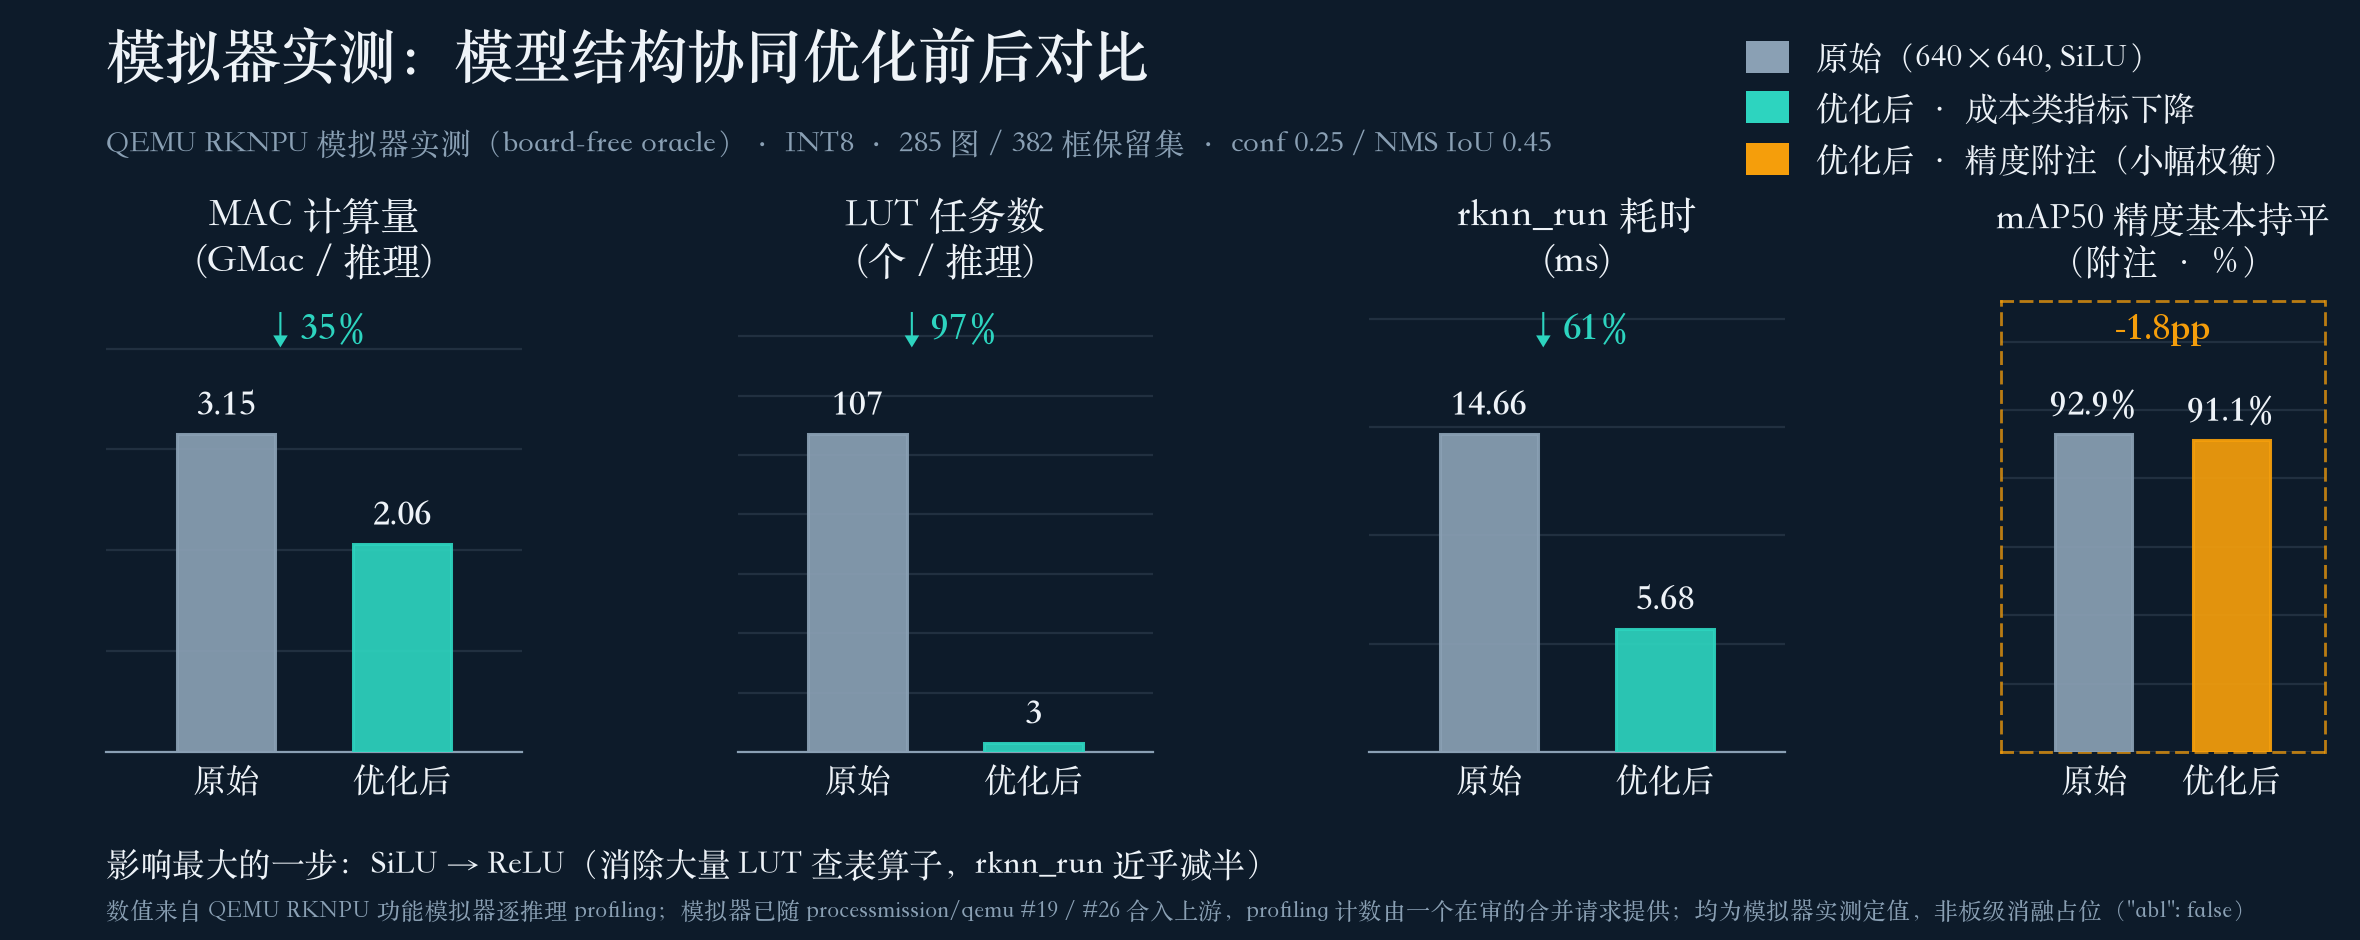
\includegraphics[width=\linewidth]{F13.png}
    \end{column}
    \begin{column}{0.43\textwidth}
      \begin{itemize}
        \item 本队将闭源 RK3588 RKNPU 实现为功能级 QEMU 模型（qemu\#19、qemu\#26，106 qtests），真实执行 INT8/FP 并接入 IOMMU
        \item 模型将板上调试的加速器转为 board-free、寄存器精确的开发、CI 与优化载体
        \item 逐层重塑网球检测模型：输入缩放与 SiLU 改 ReLU 累计使 LUT 任务 107$\to$3、rknn\_run 减半，叠加类别头收窄、头框合并（左图为模拟器实测，非真机）
      \end{itemize}
    \end{column}
  \end{columns}
  \advance{加速器闭源、原本只能板上调试}{QEMU RKNPU 功能模型上测得模型协同：rknn\_run 降至约三分之一、精度基本持平}
\end{frame}

% ============================== B 显示与板级广度 ==============================
\begin{frame}
  \navsegment{2}
  \frametitle{显示、图形与板级：从零打通的广度}
  \begin{columns}[T]
    \begin{column}{0.32\textwidth}
      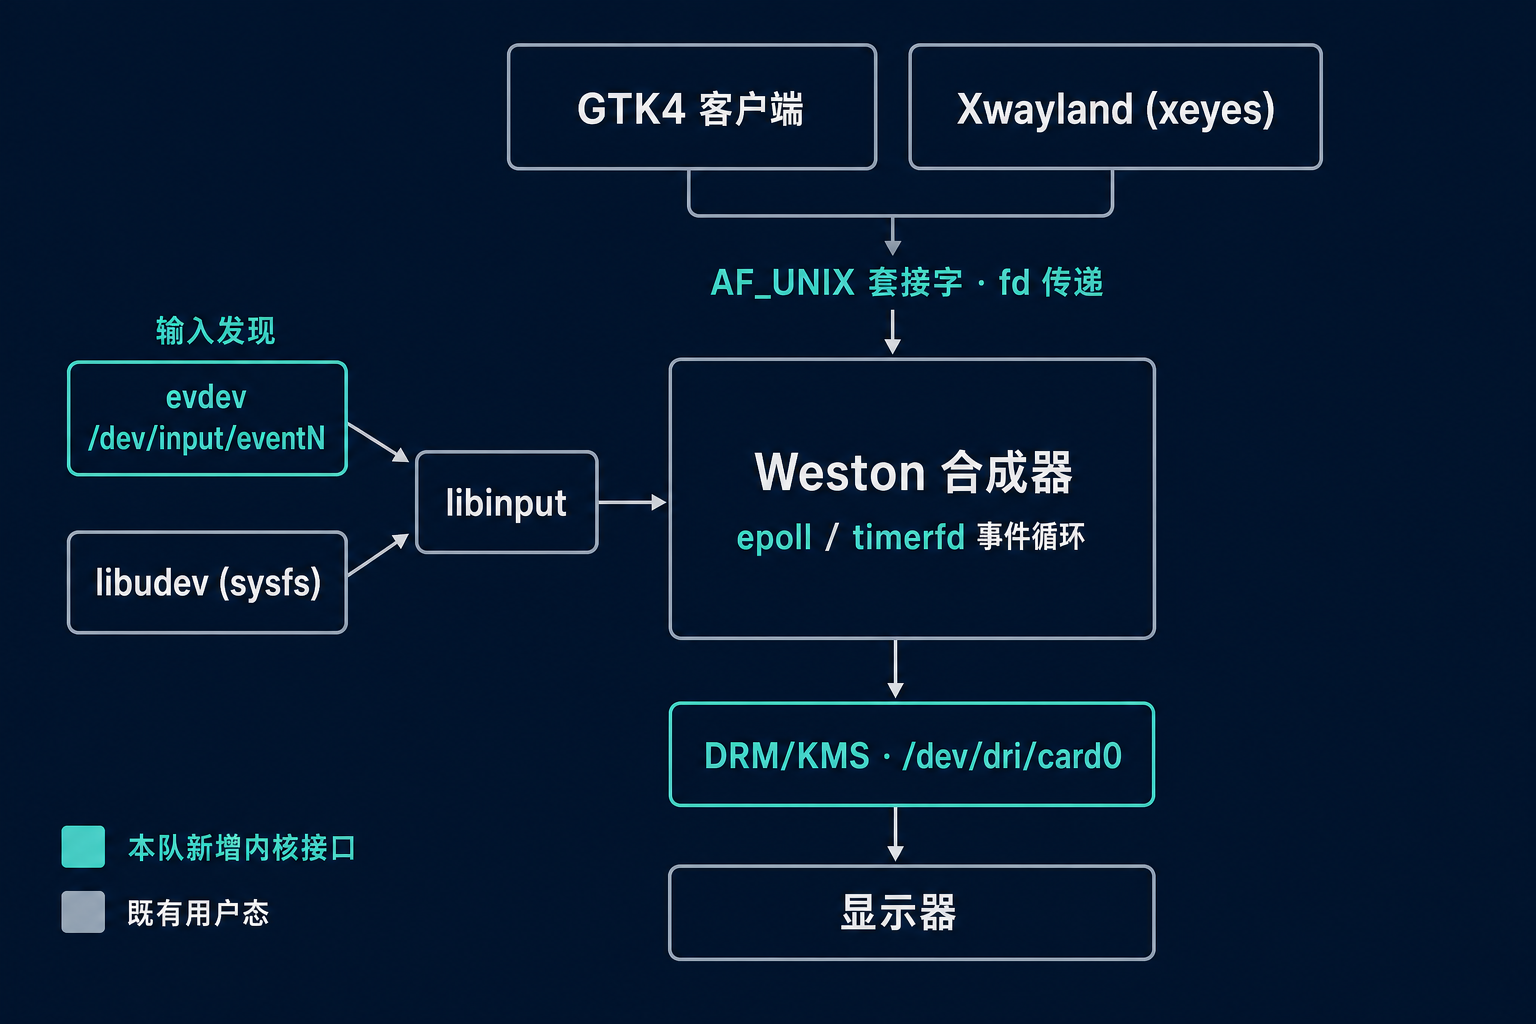
\includegraphics[width=\linewidth]{Fwayland.png}
    \end{column}
    \begin{column}{0.64\textwidth}
      \begin{itemize}
        \item \headline{原生显示栈}\ 从零实现 VOP2 + HDMI-QP + HDPTX 四个 \#![no\_std] crate，Qt6 时钟经 \texttt{/dev/fb0} 上屏；\headline{上板点亮验证通过}（ROPLL 锁定、1080p60 光栅、彩条、Qt6 运行）
        \item \headline{Weston 合成器}\ 在 StarryOS 上运行 Weston：补齐 \texttt{/dev/dri/card0} 原子 KMS、多路输入、\texttt{AF\_UNIX} 传 fd、\texttt{epoll} 就绪语义，四架构验证，图形栈 \#503--516 / \#1160 已合并
        \item \headline{板级 I/O 与网络}\ UART、USB-serial tty、PWM、UVC 相机、reboot(2) 与网络驱动均合入上游；pinctrl 修正 + RTL8125 + rtnetlink 打通板上 SSH，暖重启回路秒级迭代
      \end{itemize}
    \end{column}
  \end{columns}
  \advance{性能对比需先能驱动板子}{显示栈上板点亮、Weston 正常运行、约 8 个板级驱动合入上游}
\end{frame}

% ============================== R 借鉴与创新 ==============================
\begin{frame}
  \navsegment{3}
  \frametitle{借鉴与创新：基础版本与本队增量}
  \begin{columns}[T]
    \begin{column}{0.47\textwidth}
      {\headline{站在何处（借鉴的基础版本）}}\smallskip
      \begin{itemize}
        \item 内核：\texttt{rcore-os/tgoskits} 的 dev 分支 @73409e079（StarryOS + ArceOS 组件）
        \item 机器人应用：移植自 \texttt{pengzechen/aka-rk3588}
        \item 模型转换：\texttt{airockchip/rknn-toolkit2}
        \item 每处改动首次提交即固定基线、如实标注来源
      \end{itemize}
    \end{column}
    \begin{column}{0.5\textwidth}
      {\headline{本队的创新与增量工作}}\smallskip
      \begin{itemize}
        \item 机器人视觉推理链路：端到端由落后 Linux 约 6.3 倍优化到持平
        \item 整 OS 对 Linux 逐轴对等，THP / TTFI / A55 / schbench 领先；全部拆为原子 PR 回馈上游，累计 \nPRMerged{} 个已合并、\nPRInflight{} 个在审，覆盖调度/内存/观测/驱动/显示/网络/虚拟化等子系统
        \item \headline{创新}\ QEMU RKNPU 功能级设备模型：把闭源 NPU 变为板外可开发、可 CI 的载体（106 qtest）
        \item \headline{创新}\ AI 掌控-闭环开发方法 + 带外电源自治测试台
      \end{itemize}
    \end{column}
  \end{columns}
  \advance{清楚区分借鉴与自研}{基础：tgoskits / aka-rk3588 / rknn-toolkit2；增量：机器人推理对等 + 整 OS 对等 + QEMU NPU 模型 + AI 方法}
\end{frame}

% ============================== M AI 方法与测试台 ==============================
\begin{frame}
  \navsegment{4}
  \frametitle{AI 掌控-闭环开发方法与自治测试台}
  \begin{columns}[T]
    \begin{column}{0.42\textwidth}
      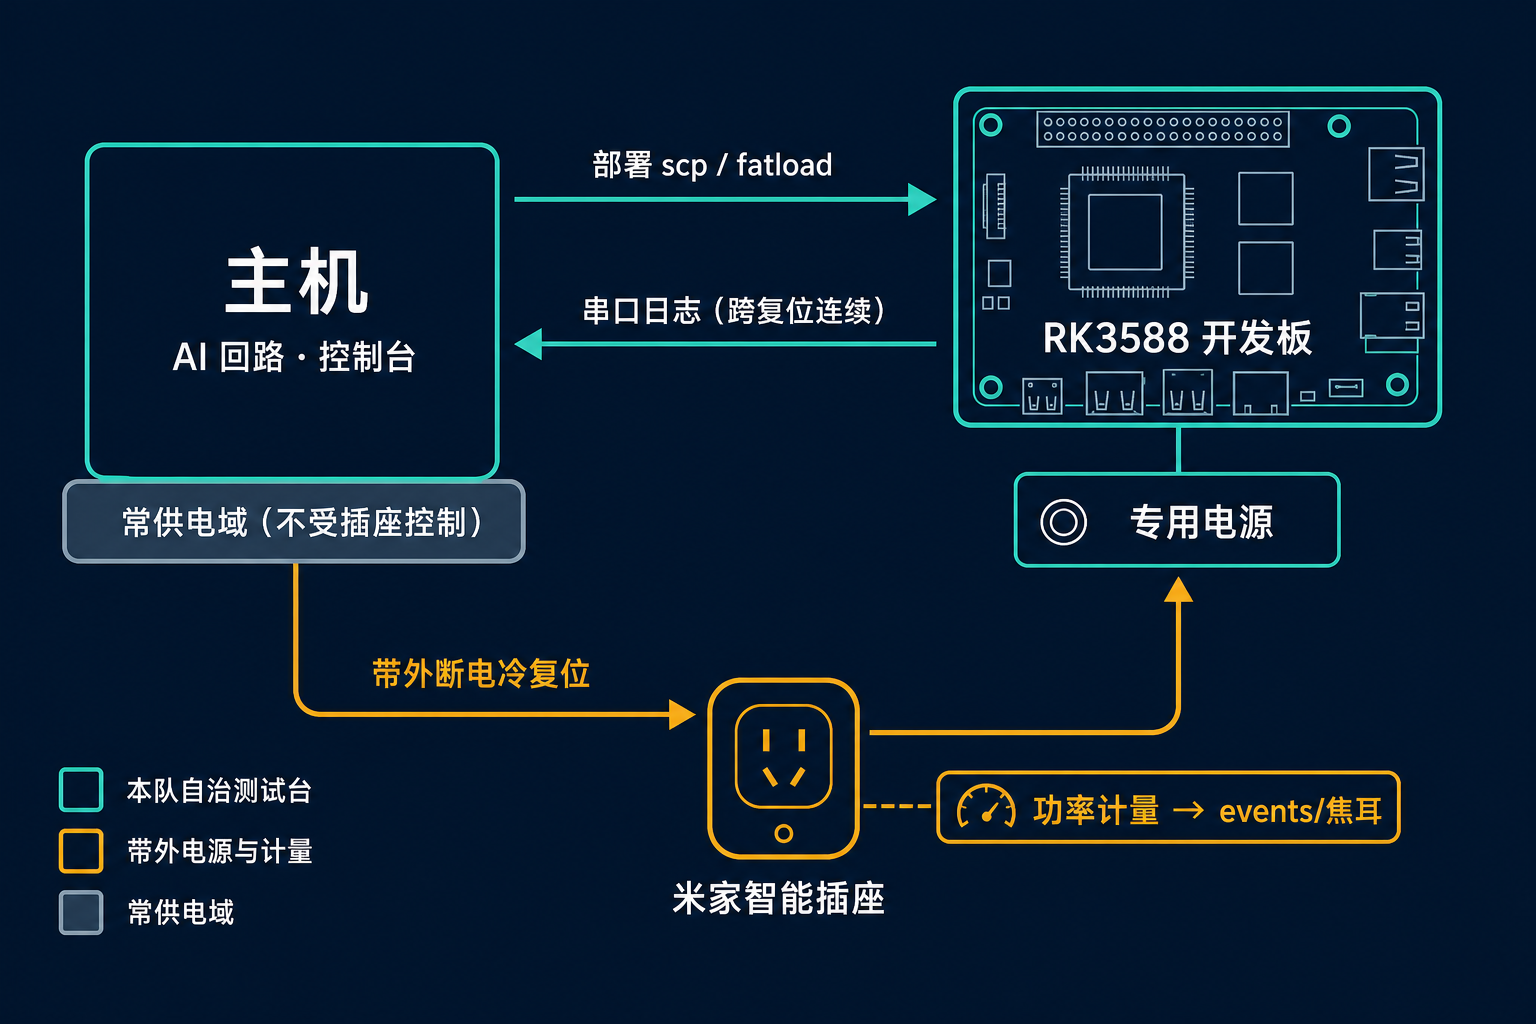
\includegraphics[width=\linewidth]{Fharness.png}
    \end{column}
    \begin{column}{0.55\textwidth}
      \begin{itemize}
        \item 人掌架构与验收，AI 在真机与 QEMU 闭环内迭代实现，运行至判定门：一次运行产出一个可由机器比对的数值
        \item 四类判定门：sysbench 对等回归、schbench 延迟阈值、多智能体对抗评审、s\_frac 计时 oracle；触及 SMP 同步的改动每次配 7 到 26 名评审
        \item 带外电源自治测试台：计量式智能插座（miIO 本地）分级恢复 L0 暖重启、L1 硬断电冷启、L2 U-Boot 黄金映像、L3 人工，令会挂死内核的改动也可无人值守
        \item 实例：cpufreq 静默吞掉电压写失败（欠压风险）经 26 人评审查出，改为失败即中止
      \end{itemize}
    \end{column}
  \end{columns}
  \advance{工作量大、共享 crate 风险高}{人掌架构、AI 闭环迭代至判定门，带外电源使真机回路无人值守}
\end{frame}

% ============================== C 小结分工与材料 ==============================
\begin{frame}
  \navsegment{4}
  \frametitle{小结、分工与材料}
  \begin{itemize}
    \item \headline{贡献小结}\ 机器人推理追平 Linux；整 OS 对 Linux 逐轴对等，THP / TTFI / A55 / schbench 领先；QEMU NPU 设备模型与 AI 开发范式；全部成果回馈上游 \texttt{rcore-os/tgoskits}，累计 \nPRMerged{} 个 PR 已合并、\nPRInflight{} 个在审
    \item \headline{分工}\ 洪世金（队长，内核性能/内存/驱动/显示）、王乙凡（QEMU NPU 模型 + 机器人应用）、徐子航（板级 I/O 与网络 + 机器人应用）
    \item \headline{后续}\ 调度全量均衡、DVFS Phase 2 电压闭环、DDR SIP 换 rkbin BL31、THP 通用化、NPU 三核上真机
    \item \headline{材料与复现}\ 同一份 ELF 两侧对照、三次重复中位数；代码见 \texttt{rcore-os/tgoskits} 与 \texttt{processmission/qemu}，报告与幻灯见 \texttt{docs/final-round/}
  \end{itemize}
  \vfill
  \centering{\sffamily\color{teal}\large Team Posad\quad·\quad 清华大学\quad·\quad 感谢 rcore-os 社区与竞赛组委会}
  \advance{开篇给出机器人与工作量}{收束：机器人对等 + 整 OS 对等 + QEMU 模型 + AI 范式；三人分工、全链可复现}
\end{frame}

% ============================== A 附录扉页 ==============================
\begin{frame}[plain]
  \vfill\centering
  {\sffamily\bfseries\color{teal}\LARGE 附录 · 备用材料}\\[8pt]
  {\color{muted}\large 目标完成表 · 基准与口径 · 增量 PR 一览 · 与类似工作对比 · 机器人状态机 · 视觉推理链路 · AI 使用说明}
  \vfill
\end{frame}

% ============================== 6 系统分层总览 ==============================
\begin{frame}
  \navsegment{0}
  \frametitle{系统分层总览与术语}
  \begin{columns}[T]
    \begin{column}{0.52\textwidth}
      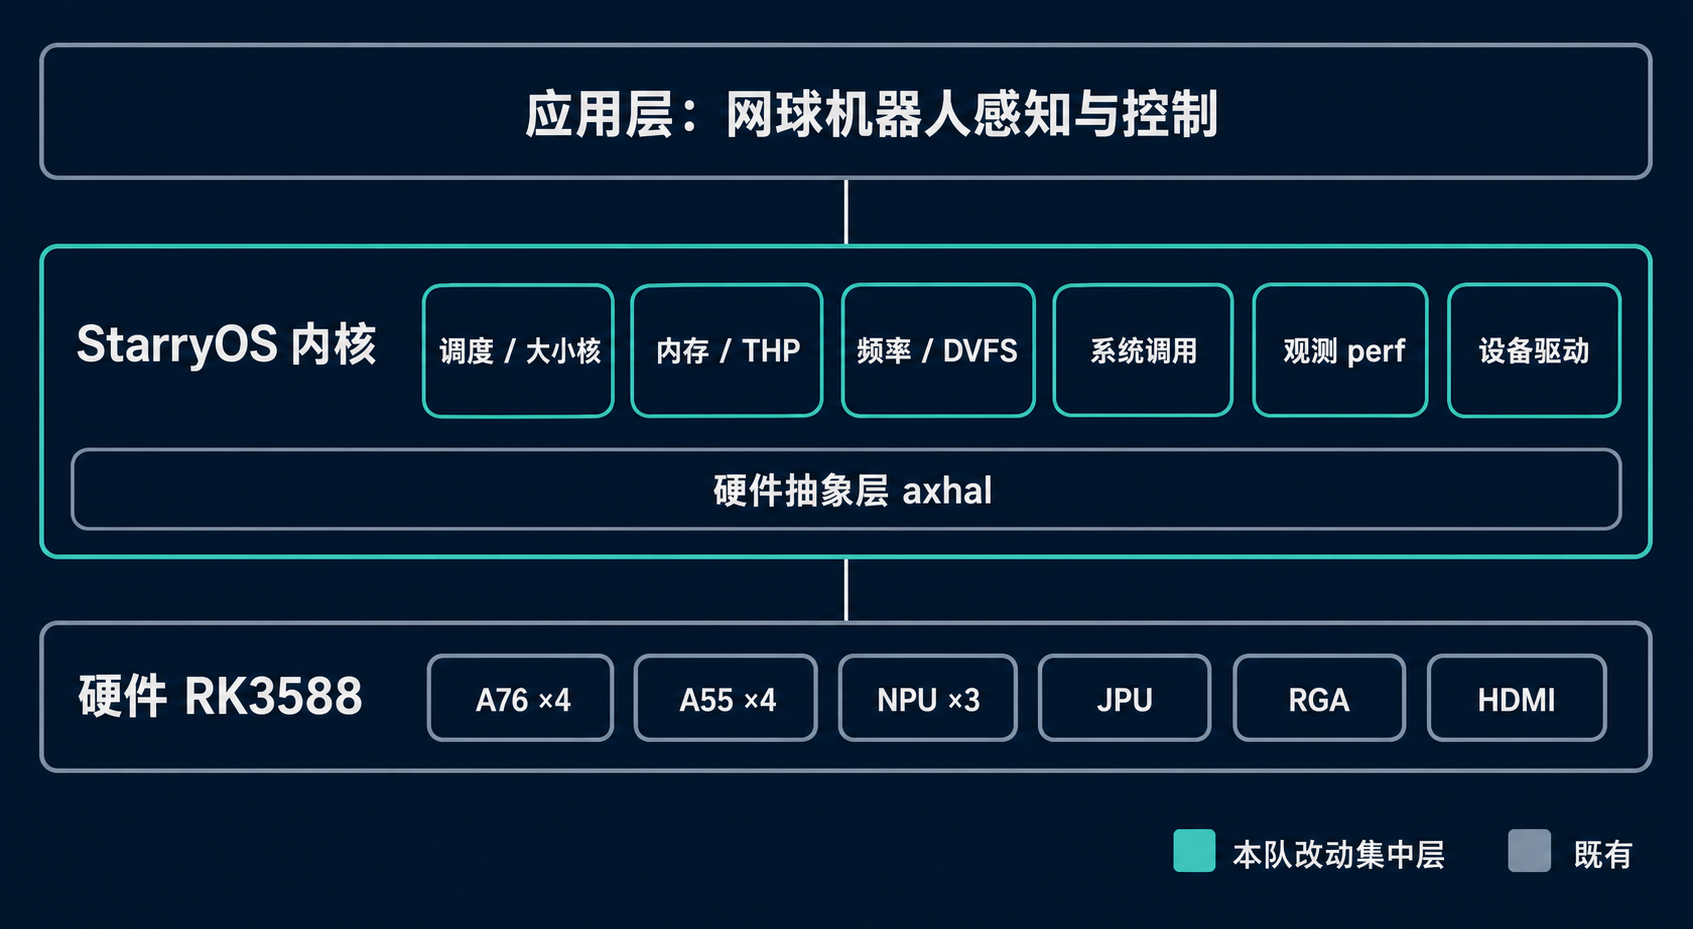
\includegraphics[width=\linewidth]{F02.png}
    \end{column}
    \begin{column}{0.45\textwidth}
      \begin{itemize}
        \item StarryOS 复用 ArceOS 模块层，补齐 Linux 兼容的系统调用、进程与信号，按设备类型分层驱动
        \item 本队改动集中于调度、DVFS、分页、观测四层，另含若干 RK3588 驱动
      \end{itemize}
      \smallskip
      {\color{muted}\footnotesize
      术语一次讲清：\\
      big.LITTLE = 4×A55 小核（cpu0-3）+ 4×A76 大核（cpu4-7）；\\
      DVFS = 动态调频调压；THP = 透明大页；\\
      TTFI = 上电到首帧推理。}
    \end{column}
  \end{columns}
  \advance{机器人回路跨越多层}{改动落在调度/DVFS/分页/观测四层，另含 RK3588 驱动}
\end{frame}

% ============================== 11 调度 核驻留 + wake_affine ==============================
\begin{frame}
  \navsegment{0}
  \frametitle{调度：核驻留与唤醒延迟}
  \begin{columns}[T]
    \begin{column}{0.54\textwidth}
      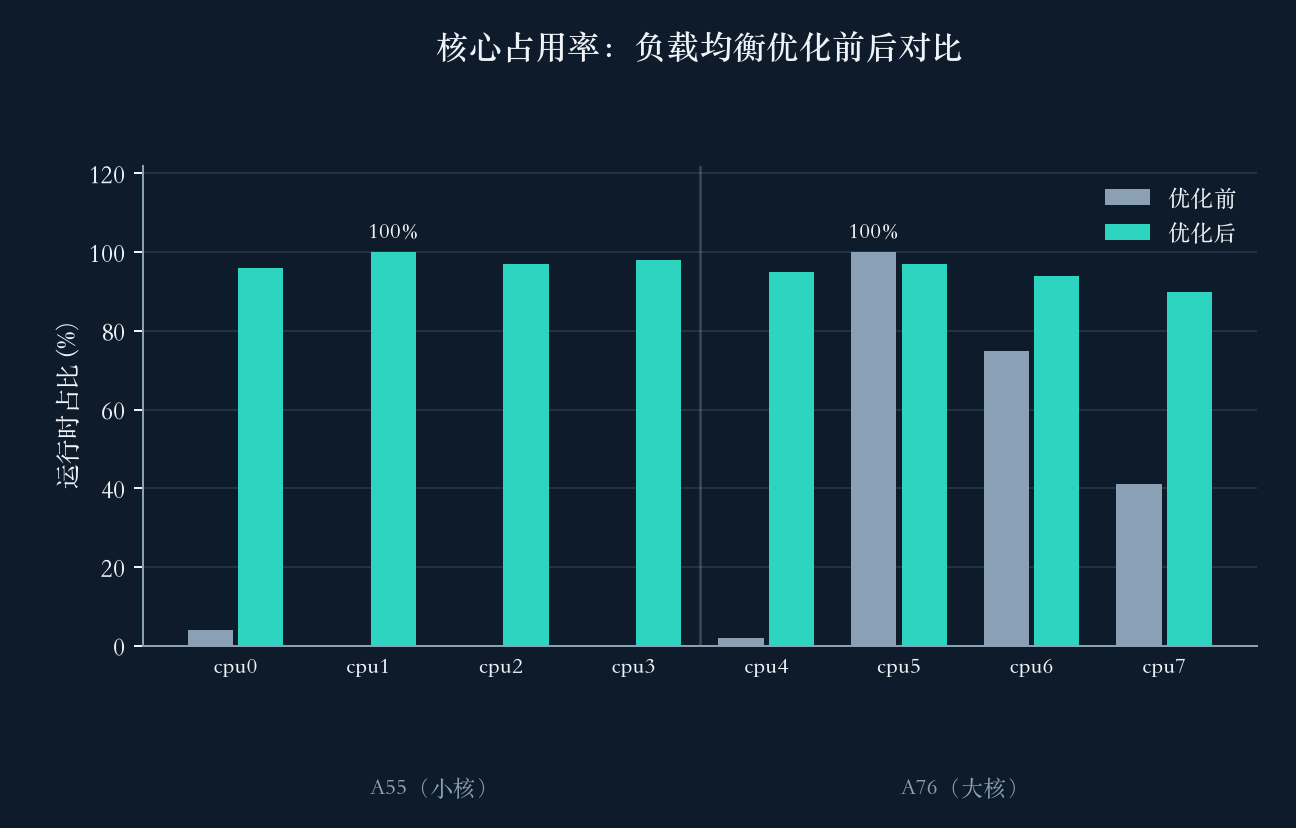
\includegraphics[width=\linewidth]{F05.png}
    \end{column}
    \begin{column}{0.43\textwidth}
      \begin{itemize}
        \item 八线程曾塌陷至 3 个 A76、A55 全程空闲，根因为唤醒聚簇
        \item 对齐 Linux \texttt{select\_idle\_sibling}：仅 occ==0 时保留 last\_cpu，否则选最空闲核，驻留随即均匀
        \item \texttt{wake\_affine} 将 m1t4 唤醒 p50 由 1042 降至 \nWake\,µs，接近 Linux \nWakeLin\,µs，判定持平
        \item 出厂启用 idle-poll 后，并发工作线程经 \texttt{select\_idle\_sibling} 铺开，schbench RPS \nSchRps 反超 Linux \nSchRpsLin（\nSchRpsRatio×）
      \end{itemize}
    \end{column}
  \end{columns}
  \advance{放置均衡后仍聚簇、唤醒存在下限}{驻留均匀 + \texttt{wake\_affine} 唤醒 \nWake\,µs 追平 Linux}
\end{frame}

% ============================== 15 频率电压 DVFS/PVTPLL + DDR 外因 ==============================
\begin{frame}
  \navsegment{0}
  \frametitle{频率电压：DVFS / PVTPLL 与 DDR 变频固件外因}
  \begin{columns}[T]
    \begin{column}{0.52\textwidth}
      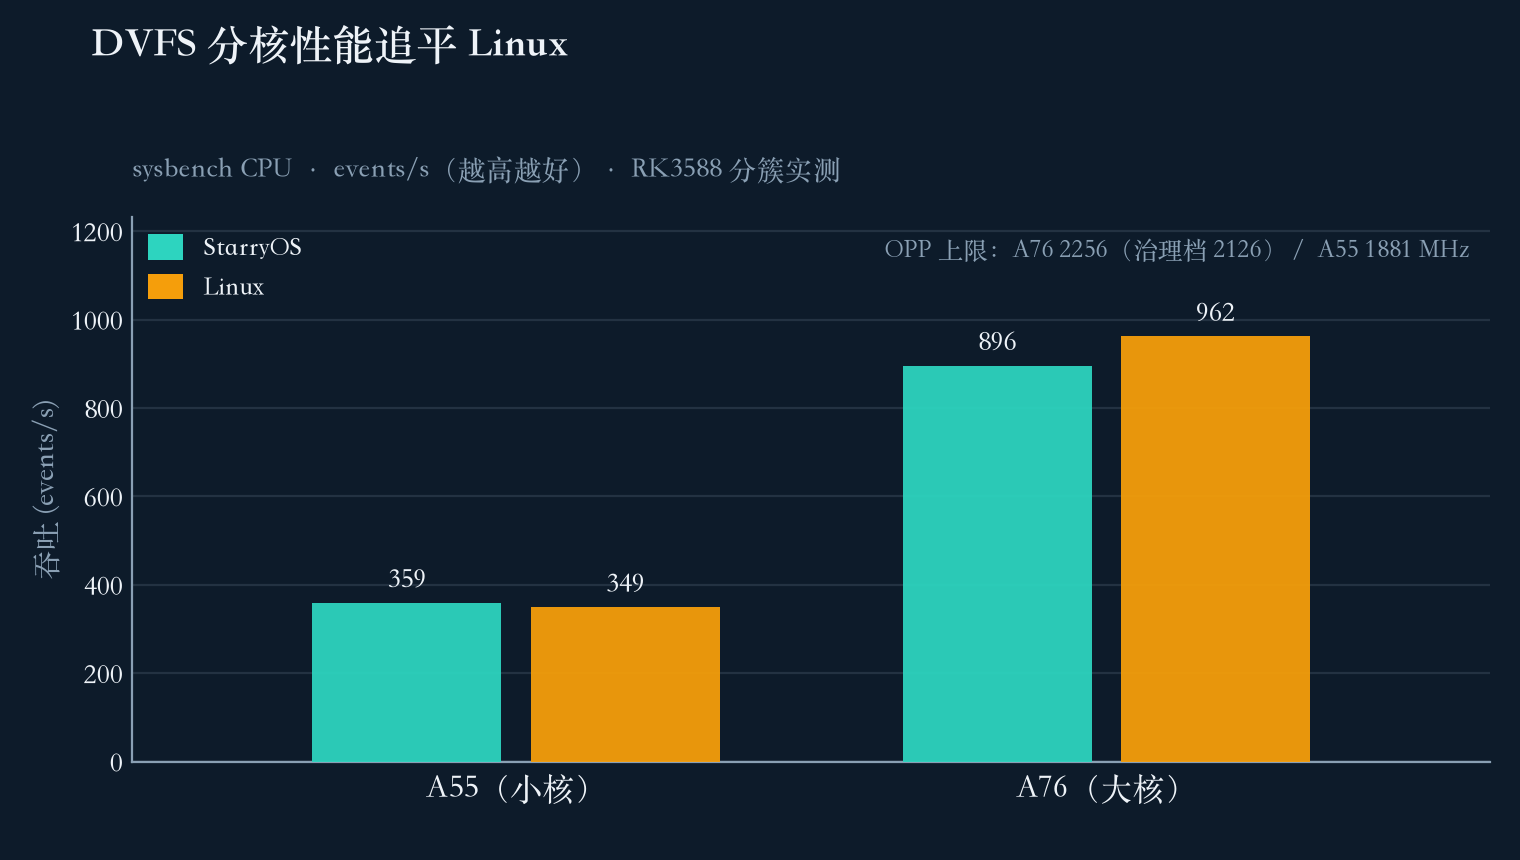
\includegraphics[width=\linewidth]{F10.png}
    \end{column}
    \begin{column}{0.45\textwidth}
      \begin{itemize}
        \item RK3588 CPU 时钟为电压耦合的 PVTPLL，频率随轨压变化，CPU CRU 由 BL31 保护
        \item \#1657：按簇 ondemand governor + PMIC 电压标定（A76 走 I2C、A55 走 SPI），事务式先电压后时钟
        \item 环长调节：更高 SCMI 速率将环由 17 重编为 11，同压更高频；A76 顶 \nDvfsAseven\,MHz、A55 顶 \nDvfsAfive\,MHz，八线程达 \nCpuTEightRatio× Linux
        \item \vwarn{DDR 变频}走 Rockchip SIP DRAM 接口，主线 TF-A 缺该 EL3 处理器，驱动已实现，停在探测态，受主线固件限制
      \end{itemize}
    \end{column}
  \end{columns}
  \advance{CPU 固定于上电低频、落后约三十倍}{ondemand + PMIC + 环长调节逐核 \nPerCoreRatio× Linux；DDR 变频受主线固件限制}
\end{frame}

% ============================== 14 页表·TLB 正确性 + blast radius ==============================
\begin{frame}
  \navsegment{0}
  \frametitle{正确性：页表与 TLB 修复的波及面}
  \begin{columns}[T]
    \begin{column}{0.5\textwidth}
      \gfxt{F09.png}
    \end{column}
    \begin{column}{0.47\textwidth}
      \begin{itemize}
        \item 提升大页、跳过失效、引入 2\,MB 块时，多代理对抗审查（每项 7 到 26 人）发现一批潜伏的 SMP 与 UAF 缺陷
        \item 主要一处：not-present 巨页块被误当页表遍历，unmap 时重复释放与 COW 共享帧构成 UAF；以 \texttt{GenericPTE::is\_table()} 统一判定修复
        \item aarch64 侧修复 PTE 写序缺 \texttt{dsb ishst}、本地 \texttt{vmalle1} 应为广播、拆分对 OOM 不原子（波及面见左图）
      \end{itemize}
    \end{column}
  \end{columns}
  \advance{THP 与跳失效改动风险面大}{对抗审查揪出 UAF 与内存序缺陷，一处修复波及三系统四架构}
\end{frame}

% ============================== 21 无收益与已回退 ==============================
\begin{frame}
  \navsegment{0}
  \frametitle{经验证暂不适用当前平台的尝试}
  \scriptsize
  \vfill
  \begin{tabular}{@{}>{\raggedright\arraybackslash}p{2.8cm}>{\raggedright\arraybackslash}p{3.1cm}>{\raggedright\arraybackslash}p{5.9cm}@{}}
    \toprule
    尝试 & 现象 & 为何无收益或回退 \\
    \midrule
    全量 work-stealing 均衡器 & 单线程 350$\to$161（0.46×），饱和无收益 & 七个空闲核反复迁移唯一工作线程，无核心保持缓存热度 \\
    自适应 haltpoll & 未稳定优于固定 50\,µs & 停机时长信号受 SGI-WFI 交互干扰而失真 \\
    early-MMU 启动重排 & 4.446 vs 4.46\,s & 低频启动窗口受 CPU 制约，缓存无从节省 \\
    第三 NPU 核 & 由两核到三核无收益 & 该模型约占一个核，增配核心无法占满 \\
    \bottomrule
  \end{tabular}\par
  \smallskip
  {\color{muted}\footnotesize 多数尝试在更换硬件类型或补足前置条件后仍有望见效，适用边界已随各条列出。}
  \vfill
  \advance{每一项改动都上板 A/B}{四条测平或测负者如实回退，并列出各自的适用边界}
\end{frame}

% ============================== 12 系统调用 getpid 微阶梯 ==============================
\begin{frame}
  \navsegment{0}
  \frametitle{系统调用入口：getpid 微阶梯}
  \begin{columns}[T]
    \begin{column}{0.54\textwidth}
      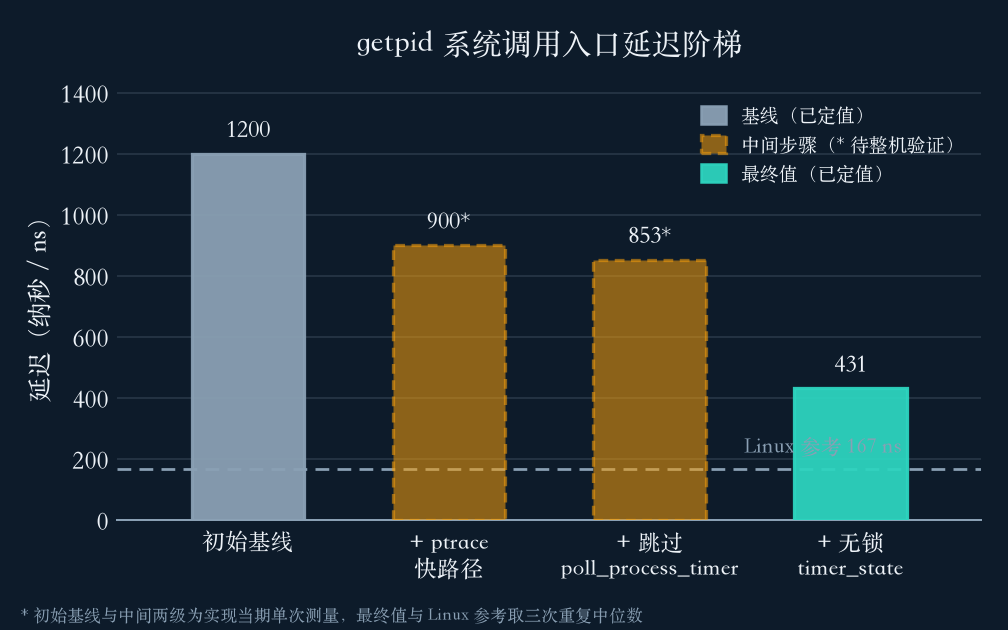
\includegraphics[width=\linewidth]{F07.png}
    \end{column}
    \begin{column}{0.43\textwidth}
      \begin{itemize}
        \item 空系统调用 getpid 基线 1200\,ns，Linux \nGetpidLin\,ns，相差约 7 倍，开销集中于进入与返回路径
        \item 三层剥离每次调用均付而多数不用的固定成本：ptrace 快路径 $-25\%$、跳过 poll\_process\_timer $-17\%$、无锁 timer\_state 粗 tick 记账 $-50\%$
        \item getpid 降至 \nGetpid\,ns，相对 Linux 由 7 倍收窄至 \nGetpidRatio 倍，stime 秒占比 0.71 对齐 Linux 0.72
        \item 残余 \nGetpid\,ns 为 \texttt{uctx.run} 陷入的架构地板，三套系统共用，无冗余可摘
      \end{itemize}
    \end{column}
  \end{columns}
  \advance{getpid 基线慢 Linux 约 7 倍}{三层剥离固定成本 $\to$ \nGetpid\,ns（\nGetpidRatio× Linux），贴陷入下限}
\end{frame}

% ============================== 20 机器人拾球应用 ==============================
\begin{frame}
  \navsegment{0}
  \frametitle{机器人拾球应用：状态机与里程计回桶}
  \begin{columns}[T]
    \begin{column}{0.34\textwidth}
      \gfxt[0.92\linewidth]{F20.png}\\[3pt]
      \gfxt[0.72\linewidth]{F21.png}
    \end{column}
    \begin{column}{0.63\textwidth}
      \begin{itemize}
        \item 应用为一份 C++ 状态机，主机 dry-run 与板端同源，仅替换电机与机械臂后端
        \item 六状态拾球闭环（追球、抓取、回桶、寻桶、趋近、投放）纯逻辑非阻塞，定时时相由单调时钟推进而与相机 FPS 解耦
        \item 里程计引导回桶：投放时 reset\_anchor 把桶设为原点，航位推算按 distance 与 bearing 回锚点，视觉一旦捕获桶即抢占
        \item 慢速轮速遥测移出控制回路，由后台线程 100\,ms 周期采样并更新位姿快照，控制回路每轮只取一次快照
      \end{itemize}
    \end{column}
  \end{columns}
  \advance{感知结果送入纯逻辑状态机}{六状态拾球闭环 + 里程计回桶，主机 dry-run 与板端同源}
\end{frame}

% ============================== 26 开发进度与完成情况 ==============================
\begin{frame}
  \navsegment{0}
  \frametitle{开发进度与完成情况}
  \begin{columns}[T]
    \begin{column}{0.54\textwidth}
      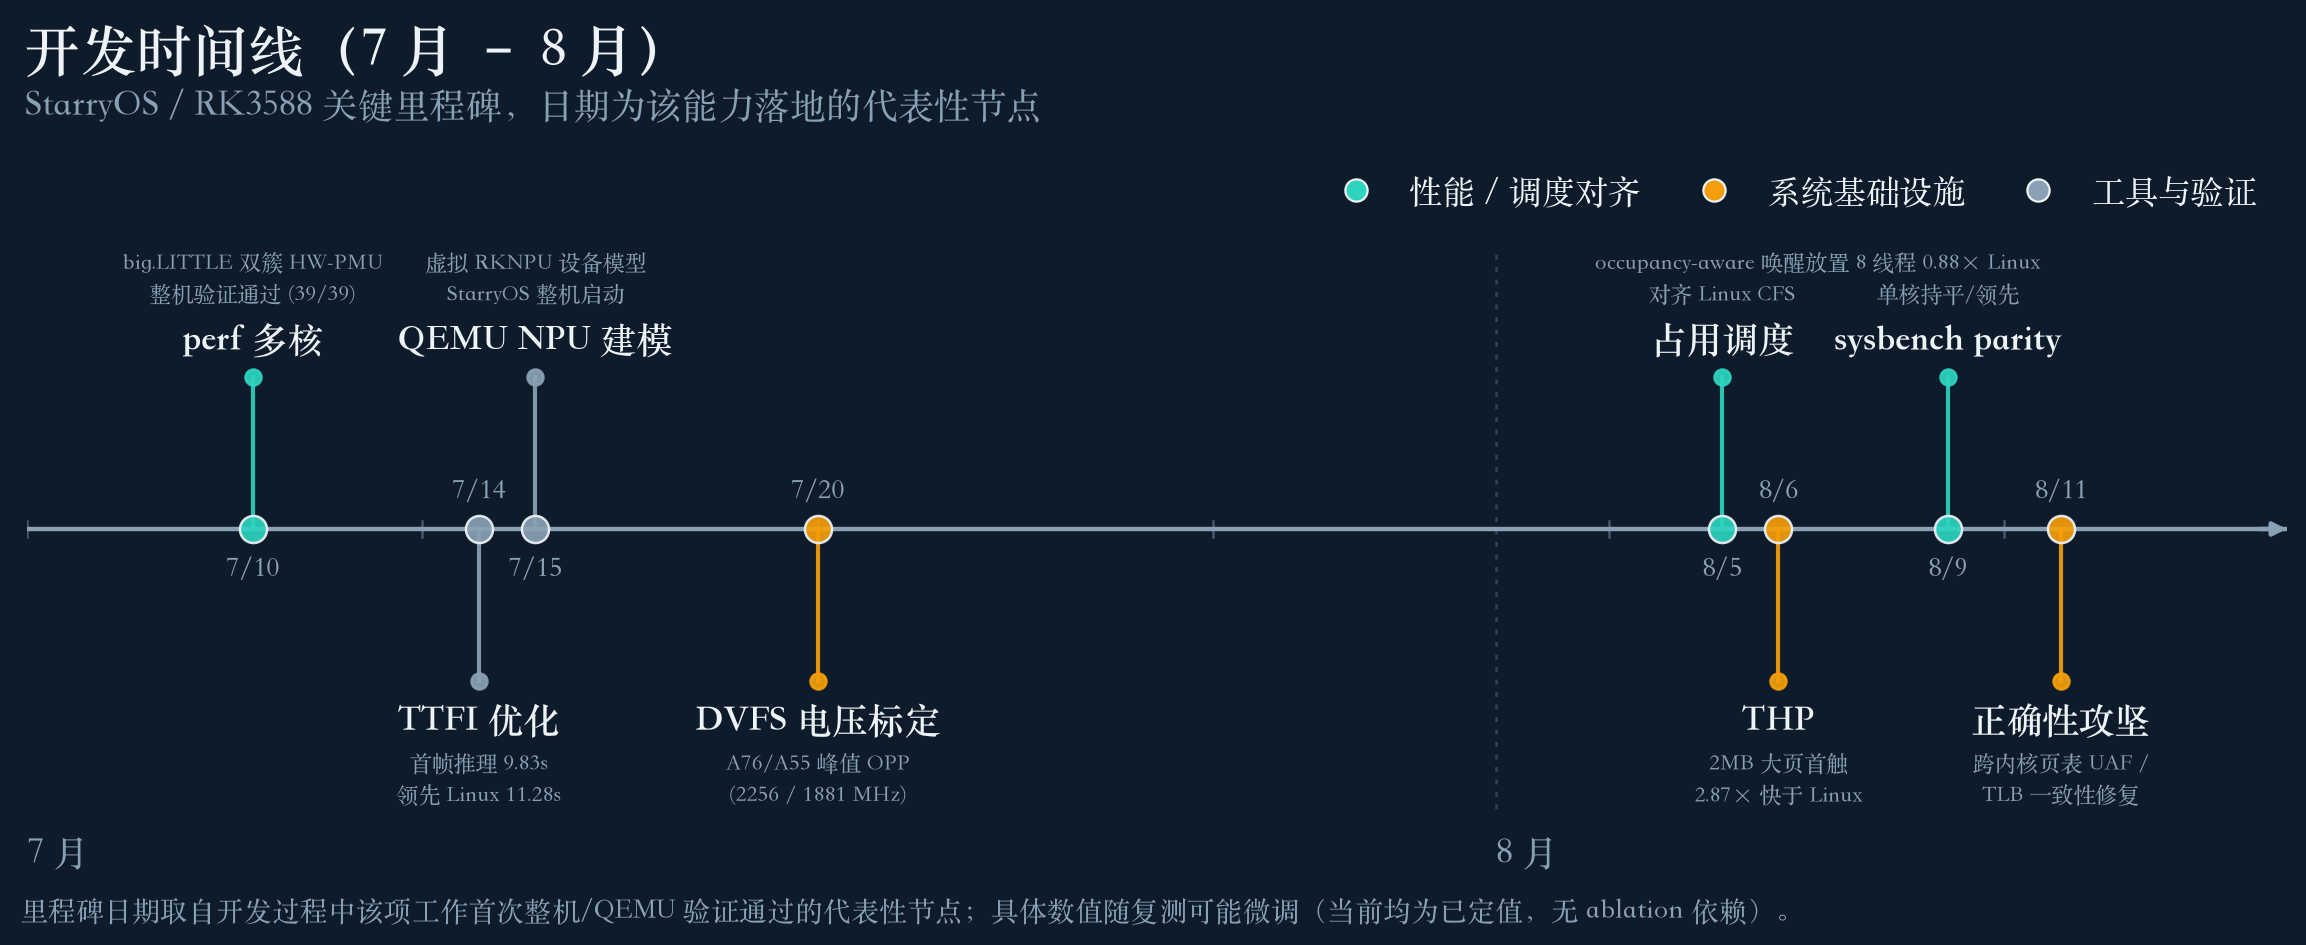
\includegraphics[width=\linewidth]{F17.png}
    \end{column}
    \begin{column}{0.43\textwidth}
      \begin{itemize}
        \item 决赛约一个月（07-01 至 08 月中），三名队员协作，各项以真板验证为准；左图为七周里程碑，自 perf 多核起至页表正确性与原子 PR
        \item 落地并验证：PMU perf、QEMU RKNPU、SMP 分布、DVFS 环长、占用调度、THP 首触、CLONE\_VM 快路径、系统调用下降、TTFI 领先
        \item 三项如实回退或受限制：工作窃取均衡器抖动回退、early-MMU 无收益回退、DDR 变频受主线固件限制
      \end{itemize}
    \end{column}
  \end{columns}
  \advance{整机对等分阶段推进}{七周里程碑，落地项均真板验证；三项如实回退或受限制}
\end{frame}

% ============================== 25 队员分工 ==============================
\begin{frame}
  \navsegment{0}
  \frametitle{队员分工（Team Posad，三名成员）}
  \footnotesize
  \begin{tabular}{@{}>{\raggedright\arraybackslash}p{2.3cm}>{\raggedright\arraybackslash}p{11.7cm}@{}}
    \toprule
    成员 & 负责模块与交付物 \\
    \midrule
    \headline{洪世金（队长）} & perf 观测（\#1395/\#1577）、调度器与大小核（\#1495/\#1656）、DVFS 与 cpufreq（\#1657）、内存与 THP、页表与 TLB 正确性、RGA2（\#1388）与 JPU（\#1456）驱动、原生显示栈 VOP2 / HDMI-QP / HDPTX、sysbench（\#1658）、报告撰写与整体协调 \\[4pt]
    \headline{王乙凡} & QEMU RKNPU 功能级模拟器：全流水线 + IOMMU + INT8/FP 执行（qemu\#19，106 qtests），多核协同（qemu\#26）；机器人拾球应用（与徐子航共同） \\[4pt]
    \headline{徐子航} & 板级 I/O 与网络：UART（\#1921）、USB tty（\#1378）、PWM（\#1468）、rtnetlink 与 SSH（\#1497）；UVC 相机（\#1924/\#1961）、reboot（\#1358）、GEM cache mmap（\#1364）；机器人拾球应用（与王乙凡共同） \\
    \bottomrule
  \end{tabular}
  \advance{三名成员按子系统分工}{队长承担内核主体，王乙凡与徐子航分担仿真板级，机器人应用共建}
\end{frame}

% ============================== 5 目标完成情况表 ==============================
\begin{frame}
  \navsegment{0}
  \frametitle{目标完成情况}
  \scriptsize
  \begin{tabular}{@{}>{\raggedright\arraybackslash}p{2.4cm}>{\raggedright\arraybackslash}p{8.3cm}>{\centering\arraybackslash}m{1.9cm}@{}}
    \toprule
    目标域 & 结果（StarryOS 优化前 $\to$ 后，对照 Linux） & 状态 \\
    \midrule
    观测 perf/ftrace & 硬件 PMU perf 与 ftrace 上板，big.LITTLE 全量通过 & \vgood{已达} \\
    调度与大小核 & cpu 八线程 \nCpuTEightBefore $\to$ \nCpuTEight\,ev/s，为 Linux \nCpuTEightLin 的 \nCpuTEightRatio× & \vgood{已达} \\
    系统调用入口 & getpid \nGetpidBefore $\to$ \nGetpid\,ns，为 Linux \nGetpidLin\,ns 的 \nGetpidRatio×（由 7× 收窄） & \vgood{已达} \\
    内存与分页 & THP first-touch \nThpFTBefore $\to$ \nThpFT\,s，Linux \nThpFTLin\,s，快 \nThpRatio×（领先） & \vgood{已达} \\
    频率电压 & CPU 调频调压经 PVTPLL 环长对齐 Linux（逐核持平）；内存写 \nMemBWWriteBefore $\to$ \nMemBWWrite\,MiB/s（\nMemBWWriteRatio×，DDR 变频属固件外因） & \vgood{已达} \\
    启动 TTFI & \nTtfiBefore $\to$ \nTtfi\,s，优于 Linux \nTtfiLin\,s（领先） & \vgood{已达} \\
    显示栈 & VOP2 + HDMI-QP + HDPTX 上板点亮，ROPLL 锁定验证通过 & \vgood{已达} \\
    QEMU NPU 模型 & RKNPU 功能级仿真合入，106 个 qtest & \vgood{已达} \\
    机器人应用 & 网球拾取机器人六状态闭环在 RK3588 真机完整运行，感知到运动控制全链路 & \vgood{已达} \\
    \bottomrule
  \end{tabular}
  \advance{决赛命题是整 OS 对等}{九个子系统的目标、结果与状态一次给全}
\end{frame}

% ============================== 8 基准套件与测量口径 ==============================
\begin{frame}
  \navsegment{0}
  \frametitle{基准套件与测量口径}
  \begin{columns}[T]
    \begin{column}{0.5\textwidth}
      \gfxt{F03.png}
    \end{column}
    \begin{column}{0.47\textwidth}
      \begin{itemize}
        \item 每个子系统采用各自业界基准，各配一条同机同频 Linux 基线，两侧运行同一份 ELF
        \item cpu 考察调度与 DVFS，memory 考察分页与 THP，hackbench 考察 fork 与并发，schbench 考察唤醒延迟，getpid 考察系统调用入口
        \item 每点取 N$\geq$5 的 p50，两次读数漂移超 $\pm$2\% 判为噪声重测
        \item 主线用累计阶梯逐层叠加，相互影响者再单独正交消融
      \end{itemize}
    \end{column}
  \end{columns}
  \advance{同一份 ELF 两侧对照}{每域一套基准 + 独立 Linux 基线 + N$\geq$5 的 p50 口径}
\end{frame}

% ============================== 23 基础版本与增量 ==============================
\begin{frame}
  \navsegment{0}
  \frametitle{基础版本与增量贡献}
  \begin{columns}[T]
    \begin{column}{0.52\textwidth}
      \gfxt{F14.png}
    \end{column}
    \begin{column}{0.45\textwidth}
      \begin{itemize}
        \item 基线冻结于 \texttt{rcore-os/tgoskits} 的 dev 分支 commit 73409e079，每处原子改动以此为起点派生为一个 PR
        \item 拆分至可独立回归的粒度，使每条改动可对照固定基线核对得失，评审仅需关注单一逻辑，触及 SMP 的改动另配多代理对抗审查
        \item 累计 \nPRMerged{} 个 PR 已合并，覆盖观测、调度、内存、DVFS、网络、驱动与外设初始化；\nPRInflight{} 个在审，含多核 perf 四件与调度分布（\#1656，把八线程由平线 \nLadderFloor{} 抬到 \nLadderPlace{} ev/s）、COW 与 THP 一组      \end{itemize}
    \end{column}
  \end{columns}
  \advance{整机对等由许多小改动累积}{固定基线，原子 PR 覆盖十余个子系统，累计 \nPRMerged{} 已合并、\nPRInflight{} 在审}
\end{frame}

% ============================== 24 与类似工作对比 ==============================
\begin{frame}
  \navsegment{0}
  \frametitle{与类似工作的对比}
  \begin{itemize}
    \item 多数 Rust OS 工作在 QEMU 或综合基准上自证，少有在真实边缘 SoC 上与同机 Linux 运行同一份 ABI 可执行文件的逐轴对照
    \item 本工作在 RK3588 真机上以同一份 ELF、同机同频、N$\geq$5 的 p50 对照 Linux，覆盖调度、系统调用、内存、频率、启动五个轴
    \item 加速器侧将闭源 RKNPU 实现为功能级 QEMU 模型（106 qtests），使 NPU 驱动与模型优化脱离板子，属可复用产物
    \item 定调诚实：给出的是对等与少数领先，并如实标注外因（DDR 固件）与后续优化方向（系统调用入口、锁竞争）
  \end{itemize}
  \advance{Rust OS 常在 QEMU 自证}{本工作在 RK3588 真机以同一份 ELF 逐轴对照 Linux，另有可复用的 QEMU NPU 模型}
\end{frame}

\end{document}
